% Theorie: Physikalische Grundlagen von Versuch/Messverfahren, Gleichungen ohne Herleitung knapp erklären
\section[Theorie]{Theorie \textnormal{\cite{paramagnet}}}
\label{sec:theorie}

\subsection{Magnetismus und Materie}

Der im Vakuum geltende Zusammenhang zwischen magnetischer Flussdichte $\symbf B$ und magnetischer Feldstärke $\symbf H$
\begin{equation}
	\symbf B = \mu_0 \symbf H
	\label{eqn:vakuum}
\end{equation}
muss unter Anwesenheit von Materie um die Magnetisierung $\symbf M$ zu
\begin{equation}
	\symbf B = \mu_0 \symbf H + \symbf M
	\label{eqn:materie}
\end{equation}
ergänzt werden. Dabei beschreibt $\mu_0$ die magnetische Feldkonstante. Verantwortlich für das Auftreten von $\symbf M$
sind atomare magnetische Momente im betrachteten Material. Daher lässt sich die Magnetisierung mit dem mittleren
magnetischen Moment $\bar{\symbf \mu}$ und der Anzahl der Momente pro Volumen $N$ als
\begin{equation}
	\symbf M = N \mu_0 \bar{\symbf \mu}
	\label{eqn:magnet_moment}
\end{equation}
ausdrücken. Ihre Abhängigkeit zu $\symbf H$ wird über
\begin{equation}
	\symbf M = \mu_0 \chi \symbf H
	\label{eqn:magnet_feld}
\end{equation}
formuliert. Der Faktor $\chi$ heißt magnetische Suszeptibilität und weist selbst komplexe Beziehungen zur Feldstärke
$\symbf H$ und Temperatur $T$ auf.

\subsubsection{Diamagnetismus}

Durch die Induktion magnetischer Momente beim Einwirken äußerer Magnetfelder tritt in allen Atomen das Phänomen des
Diamagnetismus auf. Das induzierte Feld ist dem ursächlichen dabei entgegengesetzt und schwächt so dessen Einfluss ab.
Für die Suszeptibilität muss dann $\chi < 0 $ gelten. Ideale Diamagneten werden durch Supraleiter realisiert, welche
$\chi = -1$ erreichen und das Magnetfeld in ihrem Inneren vollständig verdrängen.

\subsubsection{Paramagnetismus}

Anders als der Diamagnetismus ist der Paramagnetismus keine universelle Eigenschaft der Materie, sondern lässt sich nur
bei Atomen, Ionen und Molekülen beobachten, deren Gesamtdrehimpuls nicht verschwindet. Bei Abwesenheit eines äußeren
Feldes sind die an den Drehimpuls gekoppelten magnetischen Momente durch thermische Bewegung zufällig orientiert, sodass
keine mittlere Magnetisierung existiert. Wird jedoch ein Magnetfeld angelegt, richten sich die Momente parallel dazu aus,
sodass dessen Wirkung verstärkt wird. Die Suszeptibilität erfüllt dann $\chi > 0$ und ist aufgrund des Störeinflusses der
thermischen Bewegung temperaturabhängig. Anhand dieses Modells kann $\chi$ nun berechnet werden.

\subsection{Paramagnetische Suszeptibilität} 

Der atomare Gesamtdrehimpuls $\symbf J$ setzt sich aus Bahndrehimpuls der Elektronenhülle und Eigendrehimpuls der
Elektronen, dem Spin, zusammen. Für den Paramagnetismus kann der Beitrag des zusätzlich auftretenden Kerndrehimpulses
vernachlässigt werden. Solange das äußere Magnetfeld nicht zu stark ist, wird von LS-Kopplung mit
\begin{equation}
	\symbf J = \symbf L + \symbf S
	\label{eqn:kopplung}
\end{equation}
ausgegangen, also der Annahme, dass $\symbf J$ der Vektorsumme von Gesamtbahndrehimpuls~$\symbf L$ und Gesamtspin
$\symbf S$ entspricht. Dabei setzen sich $\symbf L$ und $\symbf S$ nach
\begin{align}
	\symbf L = \sum_i \symbf l_i && \symbf S = \sum_i \symbf s_i
	\label{eqn:einzel}
\end{align}
aus der jeweiligen Vektorsumme der Einzeldrehimpulse sämtlicher in der Hülle enthaltenen Elektronen zusammen. Anwenden
quantenmechanischer Mittel liefert dann die zugehörigen magnetischen Momente, welche sich auf
\begin{align}
	\symbf \mu_L &= - \frac{\mu_B}{\hbar} \symbf L \label{eqn:mu_L}
	\shortintertext{und}
	\symbf \mu_S &= - g_s \frac{\mu_B}{\hbar} \symbf S \label{eqn:mu_S}
\end{align}
belaufen. Dabei entspricht $\hbar = \frac{h}{2\pi}$ der reduzierten Planck-Konstante, die mit Wirkungsquantum $h$,
Frequenz $\nu$ und Kreisfrequenz $\omega$ die Beziehung $h \nu = \hbar \omega$ erfüllt. Mit der Ladung $e_0$ und
Ruhemasse $m_0$ des Elektrons bezeichnet das Bohrsche Magneton
\begin{equation}
	\mu_B = \frac{1}{2} \frac{e_0}{m_0} \hbar
	\label{eqn:mu_B}
\end{equation}
das zur Drehimpulseinheit $\hbar$ gehörige magnetische Moment. Der Faktor $g_S$ entspricht dem gyromagnetischen
Verhältnis des freien Elektrons.

\begin{figure}[H]
	\label{fig:diagramm}
	\centering
	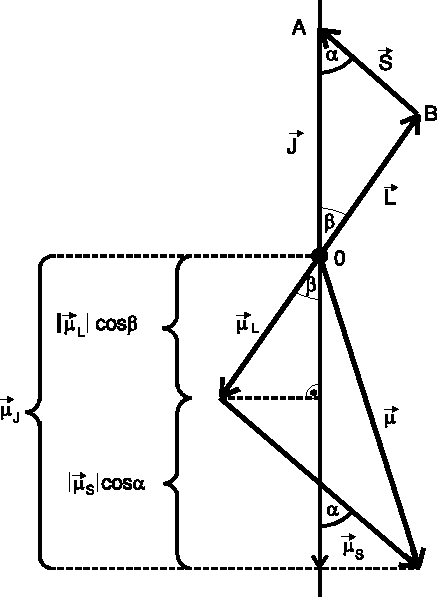
\includegraphics{content/diagramm.pdf}
	\caption{Vektordiagramm aus den Drehimpulsvektoren einer Elektronenhülle und den daraus resultierenden magnetischen
		Momenten.}
\end{figure}

\subsubsection{Seltene-Erd-Verbindungen}

\subsection{Messverfahren}

\subsubsection{Apparatur zur Induktivitätsmessung}

\begin{figure}[H]
	\label{fig:schaltung}
	\centering
	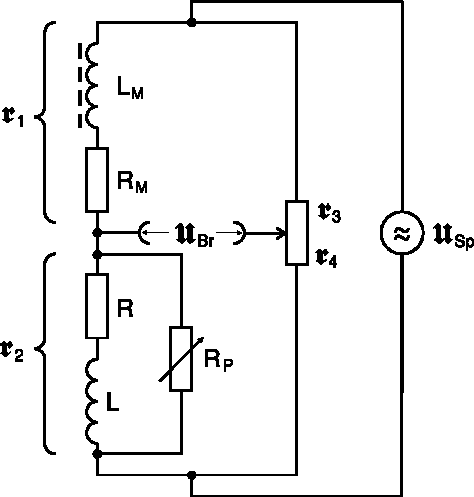
\includegraphics{content/schaltung.pdf}
	\caption{Brückenschaltung für eine Suszeptibilitätsmessung.}
\end{figure}

\subsubsection{Unterdrückung von Störspannungen}

\begin{figure}[H]
	\label{fig:kurve}
	\centering
	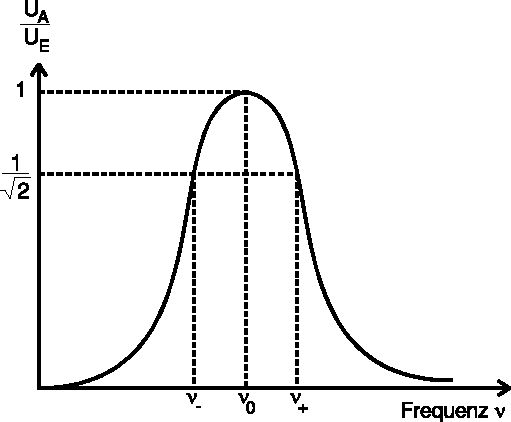
\includegraphics{content/kurve.pdf}
	\caption{Filterkurve eines Selektivverstärkers.}
\end{figure}

\begin{figure}[H]
	\label{fig:schaltbild}
	\centering
	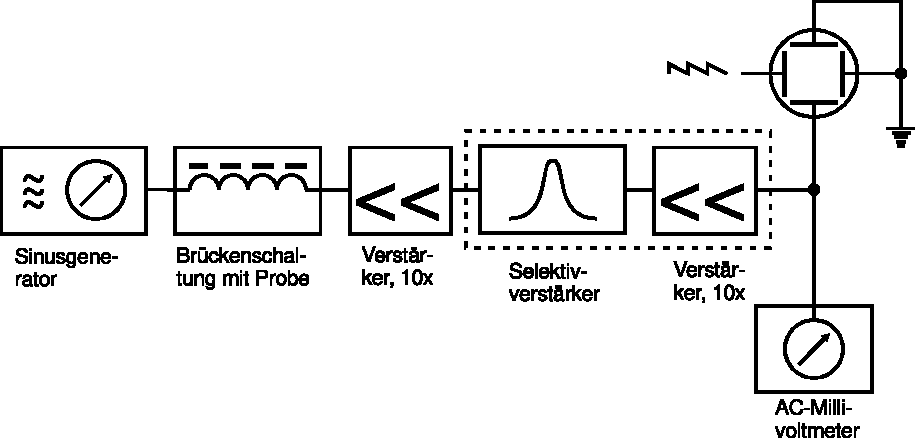
\includegraphics{content/schaltbild.pdf}
	\caption{Blockschaltbild der verwendeten Messapparatur.}
\end{figure}

$\symbffrak r$ \\ $\hbar$
